
\section{Political History}
Palestine, a country that is known by living in political conflict for decades.
The Zionist immigration to Palestine started in 1880's, with the ideology of rebuilding a national home for the Jewish people on their ancient land, the land of Israel, in Zionist parlance\citep{Morris2004}\citep{Pappe2006}\citep{Khalidi2015}.
Following the first Zionist Congress in Basel in 1897 at which the idea of
establishing a Jewish state in Palestine was first mooted, the rabbis of Vienna
dispatched two representatives to investigate the suitability of the country for
such an enterprise. The men reported the result of their explorations in this cable
to Vienna:




\centerline{\textit{\say{The bride is beautiful, but she is married to another man.}}}

This cable encapsulated the problem with which the Zionist movement had to grapple from the beginning: an Arab population already lived on the land on which the Jews had set their heart. The received view is that the Zionist movement, with the exception of a few marginal groups, tended to ignore the Arabs who lived in Palestine \citep{Shlaim2014}\citep{Karmi2007}.

\say{Zionism secularized and nationalized Judaism. To bring their project to
fruition, the Zionist thinkers claimed the biblical territory and recreated,
indeed reinvented, it as the cradle of their new nationalist movement. As they
saw it, Palestine was occupied by \say{strangers} and had to be repossessed.
\say{Strangers} here meant everyone not Jewish who had been living in Palestine
since the Roman period. For many Zionists Palestine was not even an 
\say{occupied} land when they first arrived there in 1882, but rather an \say{empty} 
one, the native Palestinians who lived there were largely invisible to them or, 
if not, were part of nature's hardship and as such were to be conquered and 
removed. Nothing, neither rocks nor Palestinians, was to stand in the way of 
the national \say{redemption} of the land the Zionist movement coveted} \cite[p.11]{Pappe2006}.

Simultaneously, The Arab Revolution was forming during the last decades of the 19th century to gain \say{Independence} from the Ottoman Empire. However, it became evident to some Palestinian leaders even before the First World War the potential for a future Jewish takeover of the country and the expulsion of the indigenous Palestinian people, it was recognized in the writings of the founding fathers of Zionism. Historical evidence shows that at some time between 1905 and 1910, 
several Palestinian leaders discussed Zionism as a political movement 
aiming to purchase land, assets and power in Palestine, although the 
destructive potential was not fully comprehended at that period \citep{Pappe2006}.



 In 1917 and during The First World War the British government issued Balfour declaration that  announces the support to establish a \say{National home for the Jewish people in Palestine}. In the same year the Ottoman Empire was destroyed by the First World War and Britain conquered Palestine \citep{Morris2004}.  
 
 
 
 
 
 The British Mandatory over Palestine was approved in 1923 and Palestine was under the British mandate from 1923 to 1948. The British Mandatory authorities had allowed the Zionist movement to build it's own independent region inside Palestine with a the infrastructure for a future state, by the late 1930's the Zionist leaders were able to form the abstract vision for Jewish exclusivity into concrete plans \citep{Pappe2006}.  
 
Orde Charles Wingate, is a British Army officer who made the Zionist leaders realize more fully that the idea of Jewish statehood had to be closely associated with militarism and an army, Wingate became a Zionist himself and he stared to train and teach the Jewish settlers troops combat methods to fight against local population,in 1920 he formed and established \say{Hagana} \textit{(“Defence” in Hebrew)}, the paramilitary organization of the Jewish community in Palestine. He succeeded in combining the Hagana troops with the British forces during the Arab revolution against the British Mandate. The Hagana troops got their first training of occupying a Palestinian village in 1938 jointly with the British forces attacked a village by the Lebanese borders and held it for hours\citep{Pappe2006}.\say{Moshe Dayan \textit{(an Israeli military leader and politician)}, who said: Wingate had taught us everything we know}\cite [p.112]{Fenby2018}. 

The Hagana also gained valuable military experience in the Second
World War, when many of its members volunteered for the British war
effort \citep{Pappe2006}. Two off shot paramilitary groups came out of the Hagana, Irgun and Lehi \textit{(Stern Gang)}. Irgun split from Hagana in 1931 and in 1940 Lehi split from Irgun\citep{Shlaim2014}. Both groups has been viewed as terrorist organizations or organization which carried out terrorist acts against Palestinians and British authorities\citep{Bell1976}.   


In May 1939, the British Government issued a policy paper called \say{The White Paper}, it promised the Palestine's inhabitants statehood and independence within ten years, also limiting the Jewish immigration to 75,000 for 5 years. The white paper also rejected the idea of partitioning Palestine to stop the Arab revolt that started in 1936 \citep{Morris2004}\citep{Fenby2018}.

That wasn't in favour of the Jewish Agency. Therefore, the Jewish Agency began to consider military action as pressure mounted within the Haganah to strike at the British. The Haganah remained cooperative with the British. But the Irgun and Lehi, launched a rebellion against British rule in 1944. They attacked police and government targets in response to British immigration restrictions. 
Apparently Lehi(Stern Gang) was desperate to achieve the Zionist dream, thus Stern before he knew that hitler is exterminating the Jews in Europe, offered an active participation and help for Nazi Germany to defeat the British and drive them out of Palestine, later on, this proposed alliance with Nazi Germany cost Lehi and Stern much support \citep{Shlaim2014}\citep{Heller1995}\citep{Grob-Fitzgibbon2011}. 

After the facts of exterminating the Jews at the concentration camps in Nazi Germany, the Irgun and Lehi intentionally avoided military targets, to ensure that they will not hamper the British war effort against their common enemy, Nazi Germany. After Nazi Germany was defeated at The Second World War in 1945, the Haganah, Irgun, and Lehi joined together as the Jewish Resistance Movement, under which they worked under a unified command structure consisting of members of all three organizations and coordinated their activities. The Haganah also lent the Irgun command of 460 Palmach fighters \textit{(Elite fighting forces of Haganah)} and provided it with funding. While the Irgun and Lehi would continue to pursue a full-scale revolt against the British, the Haganah envisioned a more limited campaign to pressure the British into acceding to Zionist demands, tying attacks mainly to targets involving the issue of immigration \citep{Bell1976}\citep{Shlaim2014}.

However, the Jewish illegal immigration to Palestine continued despite the white paper orders which it increased after the Holocaust, the Zionist groups in Europe established a well organized system for Jewish immigrants to go to Palestine Between November 1931 and December 1946, 350,800 Jews immigrated to Palestine\citep{Grob-Fitzgibbon2011}\citep{Heller1995}.   

Lehi and Irgun continued their terrorist attacks against the British authorities in multiple locations in Europe and in Palestine: exploding The British Embassy in Rome, bombing the British Colonial Club in London, Tel-aviv car park attack against the British 6th Airborne division, exploding the British police station in Haifa with a truck bomb and The King David hotel explosion\citep{Bell1976}. But the British reacted mildly, especially in comparison with the brutal treatment they had meted out to Palestinian rebels in the 1930's\citep{Pappe2006}.
 
 
 
 
\say{The decision was made by the British Cabinet to pull out of Mandatory
Palestine and leave it to the \acrshort{un} to solve the question of its future. The \acrshort{un}
took nine months to deliberate the issue, and then adopted the idea of partitioning
the country. This was accepted by the Zionist leadership who, after
all, championed partition, but was rejected by the Arab world and the
Palestinian leadership, who instead suggested keeping Palestine a unitary
state and who wanted to solve the situation through a much longer process
of negotiation}\cite[p.40]{Pappe2006}.
 
 Meanwhile the Jewish militias received a massive number of weapons during April 1948 in a hidden shipments\citep{Morris2008}\citep{Pappe2006}. The plan for ethnic cleansing was prepared by the Haganna chiefs in early March and it was called Plan D[alet]\citep{Shlaim2014}. The objective of the plan was to clear any Arab or Palestinian element inside the country\citep{Pappe2006}\citep{Shlaim2014}.
 
Plan D[alet] had multiple operations in different dates:
Nahshon in Jerusalem (2–3 April – 20 April),
Mishmar Ha‘emek (4–15 April),
Ramat Yohanan (12–16 April),
Arab Tiberias (16–18 April), 
Arab Haifa (21–22 April,)
Operation Yiftah, in eastern Galilee (15 April – 15 May), and
Operation Ben-Ami (parts I and II), in western Galilee\citep{Morris2004}.

The British left on 15 May 1948, and the Jewish Agency immediately
declared the establishment of a Jewish state in Palestine, officially recognized
by the two superpowers of the day, the USA and the USSR\citep{Pappe2006}.
 
 According to Sa’di \& Abu-Lughod
(2007) “on the last day of the mandate, the creation of the state of Israel was proclaimed,
and the 1948 Arab-Israeli war began” \citep{Sadi2007}. 



The 1948 war that led to the creation of the State of Israel over Palestine also resulted in the devastation of the Palestinian society \citep{Sadi2007}. The day that Israel was created over Palestine, for Palestinians it was a catastrophe \textit{(“Nakba” in Arabic)}. At least 80\% of the Palestinians who lived in the major part of Palestine upon which Israel was established, more than 77\% of Palestine’s territory became refugees. “The lives of the Palestinians at the individual,
community, and national level were dramatically and irreversibly changed” \citep{Sadi2007}.









The “Nakba” a massive number of Palestinians were deported outside of Palestine. “Of the
1,400,000 Palestinians in the country prior to the Nakba, just 150,000 individuals were listed
as being present during the first census carried out by the new Israeli state” \citep{Sanbar2007}.

\begin{wrapfigure}{r}{0.20\textwidth} %this figure will be at the left
    \centering
    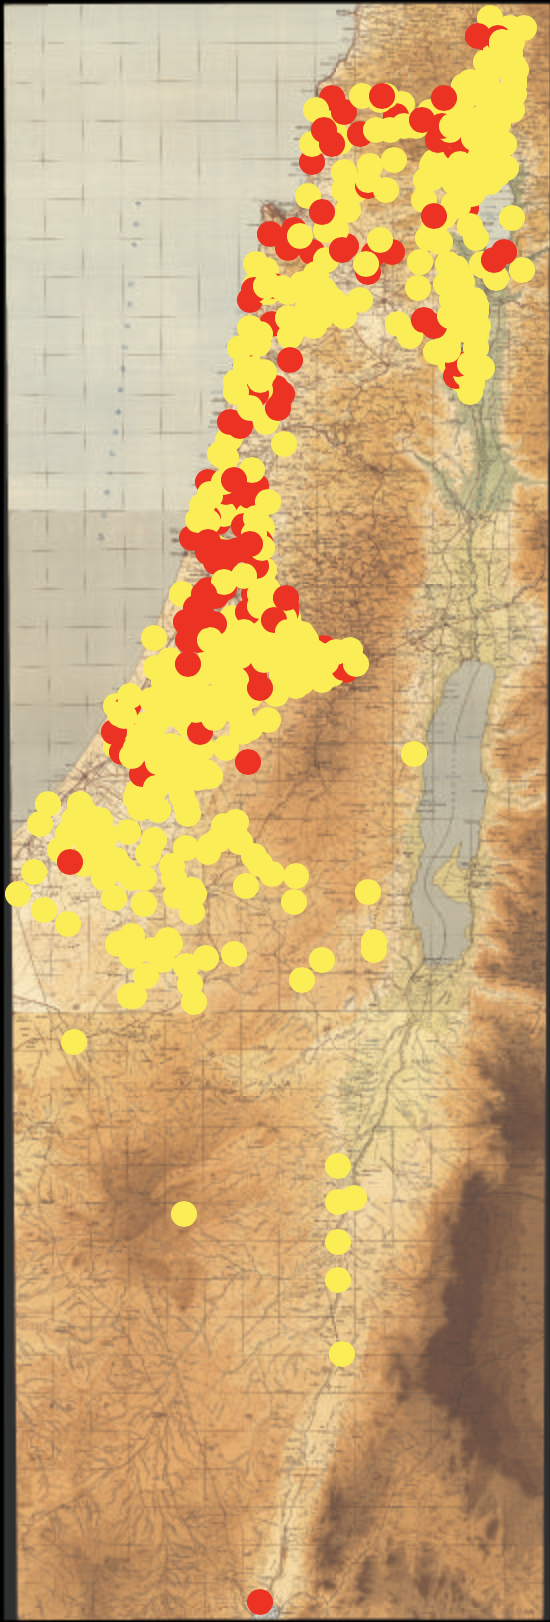
\includegraphics[width=0.20\textwidth]{d_villages}
    \caption{Demolished and depopulated villages - Palestine Open Maps, © 2018  Visualizing Palestine}
    \label{fig:map}
\end{wrapfigure}

According to Falah (1996) Some of the Israeli military code names of their operations was
Matate (Broom), and Bi’ur Chametz (Passover Cleanup) – suggest that the war involved an
aspect of ethnic cleansing \citep{Falah1996}\citep{Pappe2006}. The Israeli forces demolished and depopulated 531
Palestinian villages during the 1948 war, as shown in figure \ref{fig:map} the red dots represent the demolished villages, and the yellow dots represent the depopulated villages.  
According to the \acrshort{unrwa} in January 2015 registered
Palestinian refugees reached more than 5 million, divided between, The West Bank, Gaza
Strip, Syria, Lebanon, and Jordan \citep{Khalidi2015} \citep{DajaniDaoudi2011}. 

Since 1948 the Palestinian refugees are not allowed to return to Palestine, and not even for a visit. Due to the idea of the return of significant numbers of Palestinians to their villages and towns, or indeed to any part of Palestine, touches on deep-seated fears among Israelis regarding the legitimacy and permanence of the entire Zionist enterprise, as well as the Arab-Jewish demographic balance within Palestine \citep{Khalidi2016}.



According to Pappé (2006), the Zionist organization and the Hebrew University mapped and made a detailed registry of all the Arab villages \citep{Pappe2006}.



The project of mapping the whole villages details was funded by \textit{\acrfull{jnf}} and turned out to be a \say{national project} and it was called \say{The village files}\citep{Pappe2006}. 


In the late 1940's the \say{archive} was almost complete and the information became more explicitly military orientated \citep{Pappe2006}. In 2018 the Israeli national archive was published online, but after a time of research through the archive in English and in Hebrew, those maps and the detailed information about the villages were not openly published. According to Shezaf (2019), the Israeli defense ministry secretive security department (Malmab) is responsible for concealing hundreds of documents as a part of a systematic effort to hide evidence of the Nakba \citep{Shezaf2019}.\say{Yehiel Horev, who headed Malmab for two decades, until 2007,
acknowledged to Haaretz that he launched the project, which is still
ongoing. He maintains that it makes sense to conceal the events of
1948, because uncovering them could generate unrest among the
country’s Arab population. Asked what the point is of removing
documents that have already been published, he explained that the
objective is to undermine the credibility of studies about the history
of the refugee problem}\citep{Shezaf2019}.


\subsection{Operation Ben-Ami}

Operation Ben-Ami carried out in two stages between 13 and 22 May 1948
were specifically told that the villages had to be eliminated in revenge for the
loss of the convoy. Thus the villages of Sumiriyya, Zib, Bassa, Kabri, Umm
al-Faraj and Nahr were subjected to an upgraded, crueler version of
the 'destroy-and-expel' drill of the Israeli units. their mission is to attack for
the sake of occupation, to kill the men, destroy and set fire to Kabri, Umm
al-Faraj and Nahr \citep{Pappe2006}. The operation objective is to capture all of the villages along the coast from the south of Acre to Ras Al-naqoura in the north by the Lebanese borders and to clear it from all their inhabitants \citep{Morris2004, Morris2008}.

The Haganna troops went along the coast with armoured cars and trucks and some troops landed by boat near Sumiriyya. The Haganna  attacked Sumiriyya with mortars and left the eastern side open to allow people to flee, then the village was immediately demolished \citep{Morris2004, Morris2008}.

Bassa took more than a day to defeat due to the resistance from the village militant and some \textit{\acrfull{ala}} volunteers. The resistance gave another incitement for the Haganna to \say{punish} the village beyond expelling it's people. Haganna troops entered Bassa and ordered all the young men to be lined up and executed in front of one of the churches. After the massacre the village was totally destructed, the last village that fell in stage two of Ben-ami operation was Al-Ghabisiyya \citep{Morris2004, Pappe2006}.  



\section{Al-Ghabisiyya Village}

Al-Ghabisiyya is located north east acre in distance of 11.5 km. The village stood on a rocky hill that jutted up from the plain of Acre. Judging from the many caves that were used as burial places, the area probably had been a large Canaanite town.
Al-Ghabisiyya was populated by 690 inhabitants, in 1931 it had 125 houses. The village was built in the late nineteenth century, it was inhabited by 150 residents back then\citep{Khalidi2015}.
\subsection{Al-Ghabisiyya before 1948}

 Al-Ghabisiyya was surrounded by a variety of trees like, olives, fig, and pomegranate. The village was near another two Villages Shaykh Dannun and Shaykh Dawud. Shaykh Dawud and Shaykh Dannun were overlapped at points, but Al Ghabisiyya was about 500m away from them. The entire population of these villages was Muslim. 

Al-Ghabisiyya had a school that was built by Ottomans in 1886. The village houses were built of reinforced concrete or, in some cases, stone held together with a mortar of mud or cement. The economy of the village was based on livestock raising and agriculture, grains and vegetables were the chief crops. the villagers also grow olives, which they processed on two animal-drawn presses, one in Al-Ghabissya and one in Shaykh Dawud.

In 1944/45 a total of 6633 dunums of the lands of the three villages was allocated to cereals, 1371 dunums were irrigated or used for orchards. In the same year 300 dunums in Al-Ghabisyya were devoted to olive trees\citep{Khalidi2015}.

\subsection{Occupation and Depopulation}

Al-Ghabisiyya fell at the end of operation Ben-Ami, the Haganah's invasion of the northwest corner of Palestine. The operation, which began 13-14 May 1948, was the last major Haganah offensive before the end of the British Mandate in Palestine. It was designed to capture all the coastal villages from Acre northwards to the Lebanese border\citep{Khalidi2015}.

In the words of Israeli historian Benny Morris, this was \say{in line with Plan D[alet]'s provision for securing blocks of Jewish settlement even outside the partition plan borders.}\cite[p.252]{Morris2004}

The Carmeli Brigade which carried out the operation, was given the order on 19 May 1948, "to attack with the aim of conquest, the killing of adult males, destruction and torching villages of Al-Kabri, Umm al Faraj and Al-Nahr"\cite[p.253]{Morris2004}. Al-Kabri was occupied the following night, on 20-21 May, as part of the second stage of operation Ben-Ami. Along with a series of villages in western Galilee, north of Acre, Al-Nahr was captured 20-21 May 1948, during this second phase of the opertation. Units of the Carmeli Brigade attacked Al-Ghabisiyya it was the last village taken on 20-21 May 1948. Al-Ghabisiyya surrendered formally, the villagers greeted the troops with white flags, but Carmeli troops opened fire hitting several villagers and then excuted six more \citep{Morris2008}. Some of its population were expelled sometime during the following days or weeks\citep{Morris2004}.

The attack was waged from two directions, the north and southeast. The occupying forces captured a house in the southernmost corner of the village and proceeded to shell the village from the house, killing and injuring many of the villagers while they were fleeing. Others had been evacuated earlier, due to the fall of Acre. The village militia decided to not confront the Zionist forces because they were too few (around twenty) and very poorly armed. Most of those who were driven out remained in other villages in Galilee until the whole region fell at the end of October 1948, after that they were displaced to Lebanon\citep{Khalidi2015}.

Some inhabitants remained in Al-Ghabisiyya until Febrauary 1949. During that month, there was a second explsionm this time by the Military Government, on grounds of "security and order". it is not clear where they expelled villagers were taken\citep{Morris2004}.

After Al-Ghabisiyya and its two neighboring villages of Shaykh Dannun and Shaykh Dawud were evacuated, the Israeli government permitted some of the inhabitants of the latter two villages to return to their homes. Those who had not sought refuge in Lebanon came back and were joined by a few families from Al-Ghabisiyya, Al-Nahr, Al-Tall, Umm Al-Faraj, 'Amqa, and Kuwaykat. The two small villages of Shaykh Dannun and Shaykh Dawud were merged to form a joint village called Shaykh Dannun, in 1973 it had a population of about 1000. The Village of Al-Ghabisiyya was not repopulated \citep{Khalidi2015}.  

\subsection{The Village Today}

The only landmark that remains is the mosque, a doomed, stone structure, with arched doors and windows and decorative arches in the interior. It is deserted, the cement plaster on the doom is peeling off, and wild shrubs cover the rest of the roof. The debris of houses, terraces, and the village cemetery can be seen among a thick forest of cypress trees that was planted on the village site and part of the land. Cactus's also grow on the site. The settlement of Netiv ha-Shayyara that was established by Iraqi Jewish immigrants in 1950, uses the adjacent non-forested land for agriculture.    
\section{Current Political Context}

After 1948, The West Bank and East Jerusalem were incorporated into the Kingdom of Jordan and the Gaza strip became an Egyptian trust territory \citep{Houdaille2010}. In 1967 Israel occupied the rest of Palestine, Sinai in Egypt, and the Golan Heights in Syria by a six days war. The Palestinian Resistance movements united under the name of Palestine Liberation Organization (PLO). The national uprising (in Arabic: intifada) started inside Palestine against the occupation in 1987, where it led to peace negotiations between Yitzhak Rabin representing the Israeli government and Yasser Arafat as a representative of the PLO in 1993. The Oslo Accords is the name of the agreement that was signed between the Israeli government and the PLO, the Oslo Accords were based on the UN security council resolution 242 that proposed Israel withdrawal to the 1967 borders and the right of the Palestinian people to self-determination. It was the hope for the establishment of a Palestinian state since the Palestinians took control of some cities and areas in the West Bank and Gaza. But due to the Israeli policy of occupying more lands in the West Bank and committing violations of human rights on Palestinians that led to a second uprising (Intifada) in the year 2000 \citep{Shalhoub-Kevorkian2006}. The current situation in Palestine is a very controlled movement for Palestinians, a military checkpoint on every city entrance, and all the Palestinian areas are surrounded with a so-called separation wall. The separation wall is 3 times as long and twice as high as the Berlin wall \citep{Shalhoub-Kevorkian2006}.



\section{Cultural Identity}
 
 The dispossession of the Palestinian village population of 1948 did not involve a transient population, but an ancient indigenous farmer community that belonged to a civilization that had enriched the human heritage with its contribution in the fields of religion, literature, philosophy, architecture and the sciences. Therefore, it shouldn't be difficult to imagine the depth and the longevity of the trauma that affected the generations that were uprooted in 1948 or why their state of mind had been transmitted to their descendants in their diaspora \citep{Khalidi2015}.
 
 The children grew surrounded by the stories of their families and grandparents about their lost houses and villages and the ideal image of the Palestinian atmosphere and landscape that they were forced to leave it.  


They see their engagement in Palestine as a struggle for justice and equal 
rights for Palestinians suffering under the occupation. The relationship with Palestine has been transformed into a more 
symbolic, but nevertheless crucially important bond. The relationship that what can be called as Long-distance post-nationalism. Long-distance post-nationalism  has been triggered 
first and foremost by the continuous violence inflicted upon Palestinians. It is the very 
reaction to this violence and injustice that transforms their relationship with their 
ancestral country of origin. It is no longer only about Palestine as site of primordial 
‘roots’, but also about Palestine as a ‘cause’. While the point of engagement with Palestine begins in many cases with a personal interest and personal story,  it transforms 
the relationship with Palestine from one that could be read in national 
terms to one that can be interpreted in more universal terms as joining a struggle 
for justice.
One can speculate to what extent 
long-distance post-nationalism can co-exist with national forms of belonging to the 
national polity. While many of the second-generation research participants sympathised 
with the Palestinian struggle for independence, none of them realised their attachment 
to Palestine through direct engagement in nationalist movements or saw themselves as 
represented by Palestinian Authority. Yet, it is important to recognise how these different forms of attachment are not necessarily exclusive and could overlap with each 
other\citep{Blachnicka-Ciacek2018}.

It is possible to see the how the second-generation’s new post-nationalist conceptualization of Palestine might have the potential to universalize Palestinian 
struggle and, as such, make it inclusive and accessible to those Palestinians who might 
otherwise have felt disconnected from their parental country of origin. 

\section{New Media in Conflict}
The Palestinians are scattered in many different locations in the world, where they do not have any state of their own. The internet became the voice for the Palestinians to share their diaspora and daily life suffering stories through websites and chat rooms, the internet also revolutionized the communications between Palestinians in diaspora and in Palestine \citep{Ogunyemi2015, Aouragh2011}. Nevertheless,\say{It could help defy the repression of everyday life in Palestine by overcoming the limitations of checkpoints and occupation and thus generate feelings of ‘mobility’ and ‘political autonomy'}\cite [p.1]{Aouragh2011}.

Many Palestinian refugees want to go back to Palestine but they do not believe that they can, but the internet can that make it possible  
to avoid territorial borders and to overcome the limits, Palestinians separated by national borders and roadblocks or by geographical and political barriers were able to exhibit new modes of connectivity via innovative grassroots projects \citep{Aouragh2011}. 

According to \cite{Wulf2013} the Palestinians started to tell their story to the world using the internet in the late 1990's were it led to a new media activism \citep{Wulf2013}. Emails and Facebook are used by Palestinians to arrange demonstrations, and for providing more information and pictures to the outside world to show the struggle of the Palestinians under the Israeli occupation \citep{Wulf2013}. However, the Israeli government followed the Palestinians on the digital media platforms, for instance it requested from Facebook to delete the page \say{Third Palestinian Intifada} and from Apple to delete the \say{Third Palestinian Intifada} from the App Store \citep{Wulf2013}.      



\section{The YALLAH! Hackathon}

\acrshort{yallah!} Is a student’s exchange research program between the University of Siegen in
Germany and Birzeit University in Palestine funded by the DAAD. The program was
constructed for a collaboration between students to create social innovation projects.
In \acrshort{yallah!} 2018 there were three different projects Mobile Makerspace, VR Experience and
\acrshort{yallah!} Computer Club. The \acrshort{yallah!} program is divided into three phases: The preparation
phase (bootcamp), a research phase in Germany, and an implementation phase in Palestine.
The \acrshort{yallah!} Hackathon preparation phase
The participants of \acrshort{yallah!} learned about some research methods and how to apply them in
the projects through a boot camp week. During the boot camp, the teams took their first
steps in the projects by planning the research track, setting a research question, and building
a strategy to achieve their goals.
The Palestinian and the German students attended the boot camp separately, therefore the
boot camp took a place once in Germany and another time in Palestine. The purpose of the
boot camp was to introduce and train the participants on the research methods (such as how
to make interviews, how to take field notes, and how to observe while working in the field).
The students split up into 3 groups each group studied one method through literature and
then presented it to the other participants. By the end of the presentation, the students
discussed the method together and practiced it inside the group. The boot camp was very
good practice for the methods and emphasized the research skills of the participants. At the
boot camp in Germany, the Virtual reality project students made their first test in filming with
a 360o camera, they used the Samsung Gear 360 camera to record part of the boot camp
sessions in a purpose to use it later in the project as a testing video. Due to the average video
quality of the Samsung Gear 360 camera, the VR students added a task to their list that is to
find a 360o camera with better quality. The students also discussed the interesting spots in
Palestine related to the historical and religious places mentioned in biblical stories.
The \acrshort{yallah!} Hackathon research phase
The Palestinian students visited Germany for the research phase. The Palestinian and the
German exchange students met in Siegen, Germany for the first time. The students gathered
on the first day and had an introduction from the supervisors about the whole \acrshort{yallah!}
program in general and the research phase in Germany. After the introduction on the first
day, the teams of each project gathered and discussed their plans for the research and the
implementation phases. The VR team members discussed the kind of methods to be used in
the research, the team decided on Interviews and Thinking Aloud as methods for collecting
data from random people and from Palestinians who live in Germany. Therefore, there were
multiple tasks needed to be done by the team to start working with those methods. The VR
team split the tasks among the members: creating the interview questions guideline,
documentation, building a prototype, and logistics, for instance, to create a contact list of
interesting people to contact and have an interview with them.
After one month after the end of the research phase, the VR team had their second gathering
in Palestine to start the implementation phase. The implementation phase contained a lot of
filming in different places in Palestine. Depending on the research results and the discussion
with the team members, they created an organized plan for visiting different places in
Palestine and capturing the area using the camera. The plan included the main cities of
Palestine, famous touristic sightseeing locations and religious places since people showed
high interest to see those spots. Therefore, the team recorded in Jerusalem, Jaffa, Haifa, Acre, Ramallah, Nablus, Jericho, Hebron, and Bethlehem.

\subsection{VR Application development}